%% Title
%!!UPDATE THIS
\titlepage[of Imperial College London]%
{A dissertation submitted to Imperial College London\\
  for the degree of Doctor of Philosophy}
%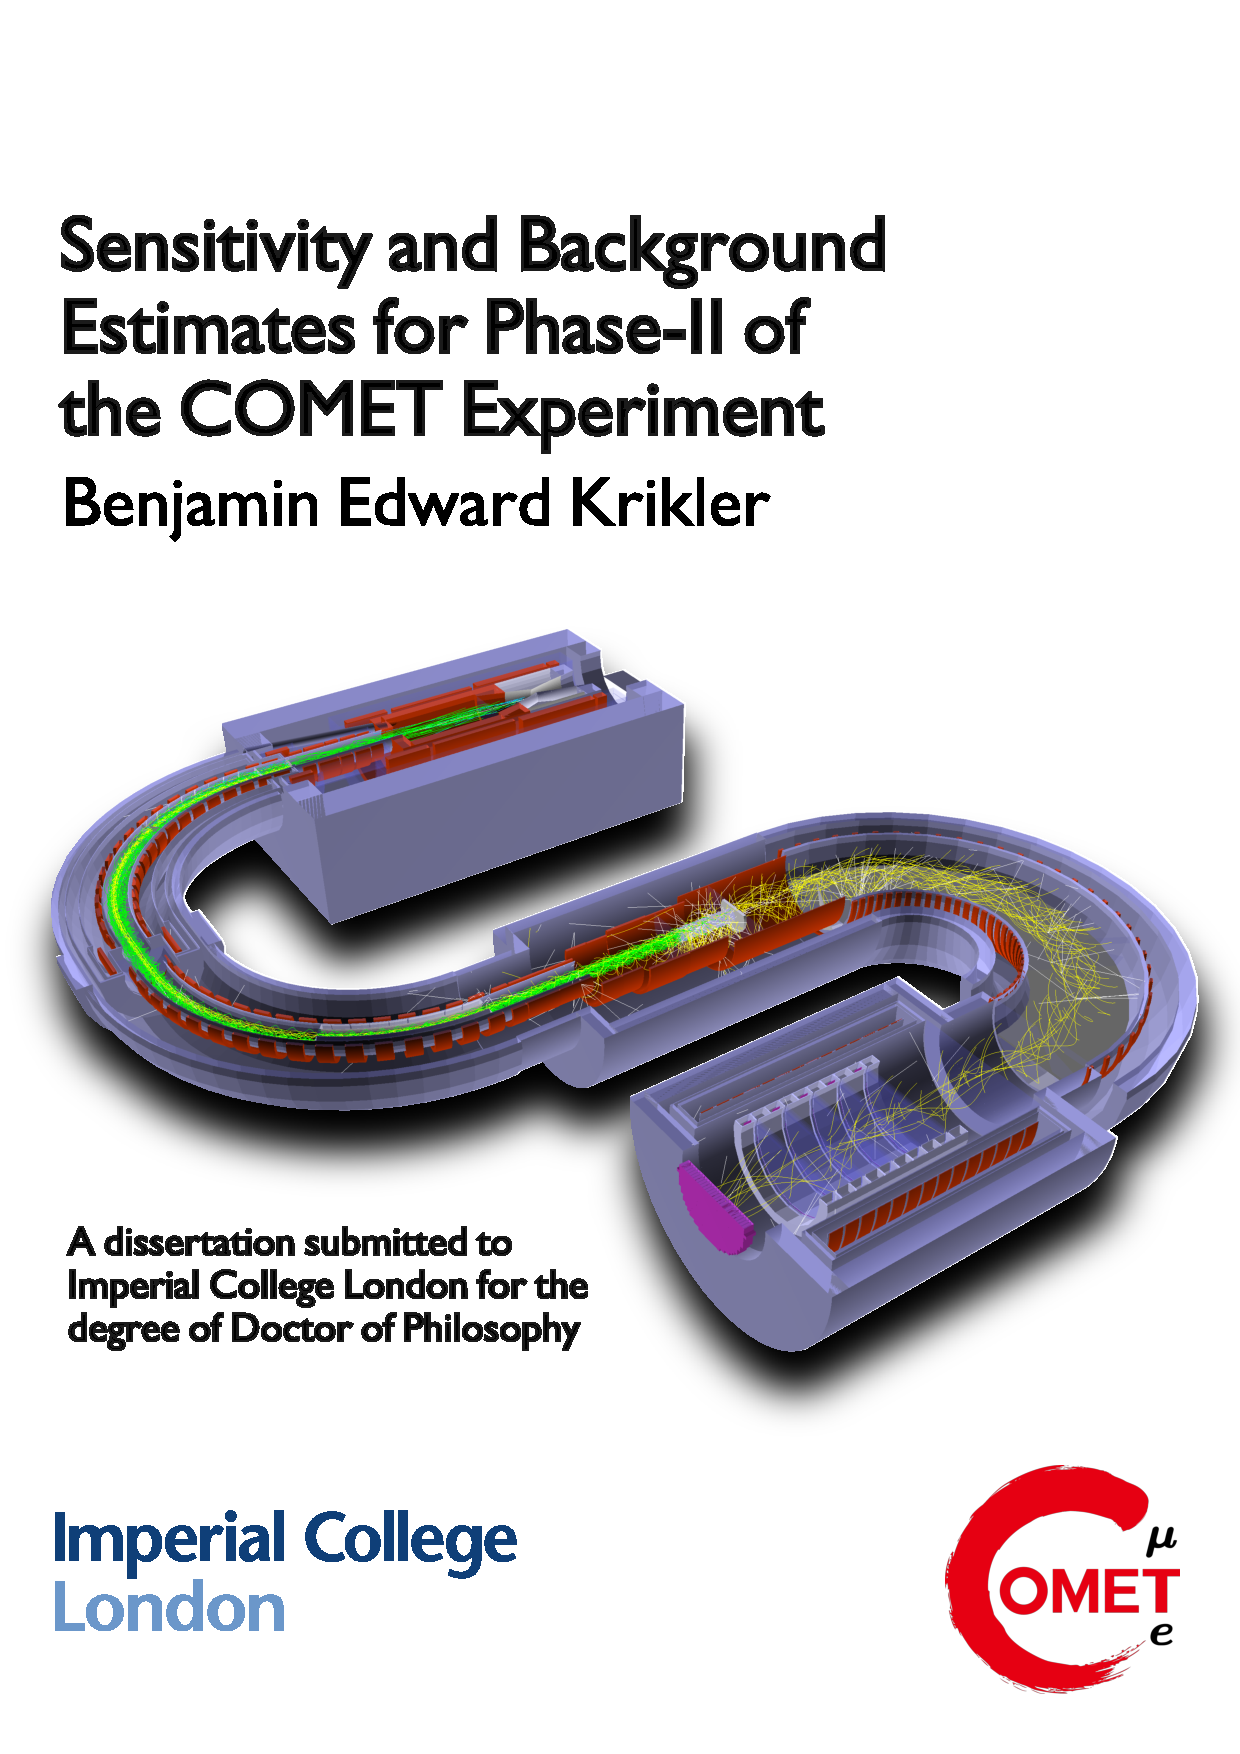
\includepdf[pages=-]{figs/FrontCover.pdf}

%% Abstract
\begin{abstract}%[\smaller \thetitle\\ \vspace*{1cm} \smaller {\theauthor}]
  %\thispagestyle{empty}
\end{abstract}

%% Declaration
\begin{declaration}
  This dissertation is the result of my own work, except where explicit
  reference is made to the work of others, and has not been submitted
  for another qualification to this or any other university. This
  dissertation does not exceed the word limit for the respective Degree
  Committee.
  \vspace*{1cm}
  \begin{flushright}
	Benjamin Edward Krikler
  \end{flushright}
\end{declaration}


%% Acknowledgements
\begin{acknowledgements}
Sir Isaac Newton is supposed to have said, ``if I have seen further than others it is by standing upon the shoulders of giants.''  
But just how tall were these giants, and what did they eat?  
How did Sir Isaac get on their shoulders and where have they all gone to?
Like many problems in physics, these are just some of the questions we still do not know.

But if this PhD has taught me anything (which I shall leave up to my examiners to decide), it is that doing science is considerably easier when working with figurative giants.
Perhaps, in the end, that is what Newton meant?  

The first of these figurative giants has to be my family.
Mum and dad, thank you for everything that you have given me, from the food, housing, clothes and the chauffering, to the curiosity and confidence to pursue what I love.
I can honestly say that without either one of you, I would be less existent.
Will and Sophie, Chris, and Marie-Claire, you are all much more recent additions to my life, but it is such a richer experience for it; I love you all.
Dan, my brother.

To Lorena, my brilliant fianc\'{e}e:
it may not be her first language, but that has certainly not stopped her correcting my english---if there are any dodgy commas in this thesis, all blame rests squarely on her shoulders.
You might have caused me to spend more time in Uberlandia, Berlin, and Amsterdam, working remotely, but then I did get to spend more time in Uberlandia, Berlin, and Amsterdam, working remotely.
Thank you for all your patience, your help, your caring; I suppose I will have to find another excuse beyond thesis stress now!

To my collaborators on COMET, it has been an absolute honour and a pleasure to work with you all.
You have given me so many opportunities to learn and grow.  
Working with collaborators from around the world has been an incredible experience in isteld.
%I have tried my best to sieze on all the opportunities you have provided me to learn and grow and mess up.
Specifically to Yoshi Kuno and Satoshi Mihara, thank you both for supporting me during my time(s) in Japan:
I do not think there are many PhD students who can say they have been driven to the airport by the spokesperson of the experiment!
To my colleagues at Imperial, in particular, thank you for putting up with my daft ideas and silly questions.
To Yoshi Uchida, my supervisor, thank you for drilling home the benefits of correct latex
The other students and the staff that I have the privilidge of being around at 
Imperial College London has provided extremely fertile ground for me, 


To my Mum and Dad, you have been 
Unfortunately, there were few giants around for me to stand on, although I have had the gigantic support of friends, family, and colleagues, without whom I could not have managed this thesis.

\end{acknowledgements}


%% Preface
%\begin{preface}
%\end{preface}

%% ToC
\tableofcontents

%% Strictly optional!
%\frontquote%
%{Light may earth's crumbling sand be laid on thee, that dogs may dig thy bones up easily.}
%{Marcus Aurelius}
%\frontquote%
%{I find it so pretentious when a thesis starts with a quote.}
%{Yoshi Uchida}
%{Writing in English is the most ingenious torture\\
%   ever devised for sins committed in previous lives.}%
%  {James Joyce}
